\documentclass[11pt]{article}
\usepackage[utf8]{inputenc}

\usepackage{hyperref}
\usepackage{wrapfig}
\usepackage{amsmath}
\usepackage{minted}
\usepackage{color}
\usepackage{svg}
\usepackage{graphicx}
\usepackage{fancyhdr}
\usepackage{rotating}
\usepackage{natbib}
\usepackage[linesnumbered,lined,boxed,commentsnumbered]{algorithm2e}

\bibliographystyle{humannat}

\graphicspath{ {./images/} }
\setlength{\tabcolsep}{10pt}
\setlength{\headheight}{15pt}

\providecommand{\shortcite}[1]{\cite{#1}}

\title{A visualiser for $\lambda$-terms as rooted 3-valent maps}
\author{George Kaye}
\date{March 2019}

\makeatletter

\pagestyle{fancy}
\fancyhf{}
\fancyhead[R]{\textsl{\rightmark}}
\fancyfoot[C]{\thepage}

\renewcommand{\footrulewidth}{0.5pt}

\begin{document}

\input{titlepage.tex}

\tableofcontents

\newpage

\section{Abstract}
\label{sec:abstract}
Todo


\subsection*{Note on the content of this report}
Some of this report (most notably the Background section) has been based on the content written in my Scientific Paper (\cite{scientificpaper}) from November.

\newpage

\section{Acknowledgements}
\label{sec:acks}
Todo


\newpage

\section{Introduction}
\label{sec:intro}

This report details the development of a set of tools to aid in the research of the topological properties of $\lambda$-terms when they are represented as rooted maps.

\subsection{Motivation}
There are many links between the $\lambda$-calculus and areas of mathematics and computer science. One such area is graph theory -- we can draw $\lambda$-terms as rooted maps and observe how the topological properties of these maps link with the computational and logical properties of the original terms.

However, performing experimental mathematics with $\lambda$-terms and their maps can be a time-consuming and boring process. The main motivation of this project was to develop tools to make this process easier and eliminate the less interesting aspects. There were two tools developed a \textbf{$\lambda$-term visualiser} and a \textbf{$\lambda$-term gallery}.

\subsection{\texorpdfstring{$\lambda$}{lambda}-term visualiser}

Drawing $\lambda$-terms maps by hand can take a while, especially for large terms. The first tool can generate maps for $\lambda$-terms from user input, in addition to providing interesting properties such as crossings. By visualising the $\lambda$-terms it can become much easier to understand the structure of more complex structures implemented in the $\lambda$-calculus (such as pairs).

The visualiser also has functionality relating to the normalisation of terms. The $\beta$-redexes contained within the term are listed, and by clicking on these the user can reduce the term to its normal form (if one exists). A normalisation graph can also be generated, which can also be interesting to examine.

\subsection{\texorpdfstring{$\lambda$}{lambda}-term gallery}
When studying properties of $\lambda$-terms, it can be useful to generate terms and look for interesting properties shared between terms and their maps. However it can be tricky to come up with terms with certain properties (such as terms containing a certain amount of subterms) on the fly. The $\lambda$-term gallery can generate all terms of a certain size and free variables, with the ability to filter based on properties such as crossings or $\beta$-redexes. This makes disproving conjectures by finding counterexamples a much easier process.

From the gallery, the user can inspect the generated terms using the visualiser, with the same functionality present as detailed above.

\begin{figure}
    \centering
    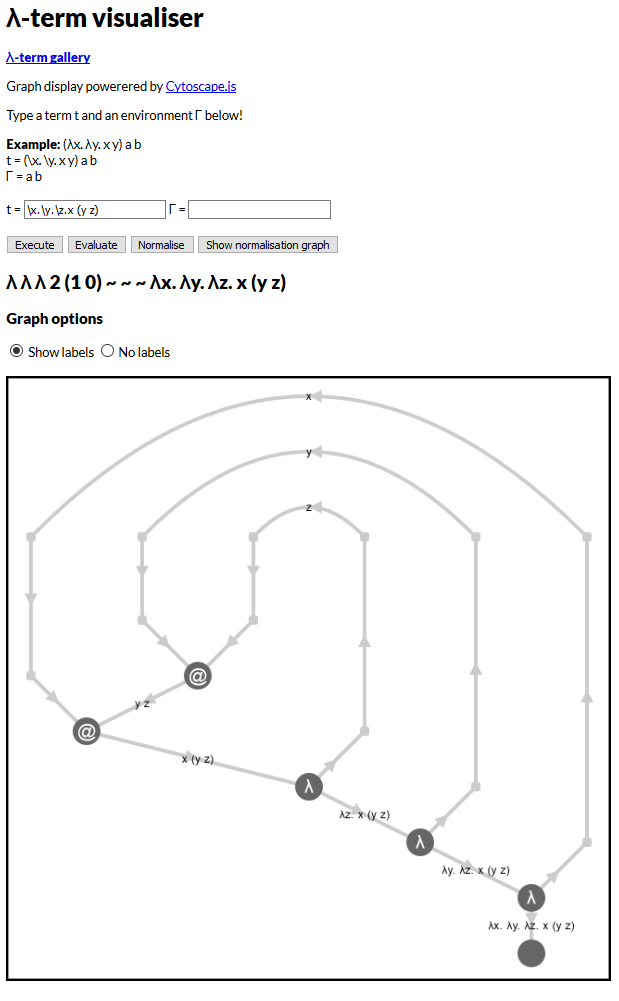
\includegraphics[scale=0.3]{visualiser}
    \caption{The $\lambda$-term visualiser, displaying the map for the term $\lambda x. \lambda y. \lambda z. x \, (y \, z)$, along with some statistics on the right.}
    \label{fig:visualiser}
\end{figure}

\begin{figure}
    \centering
    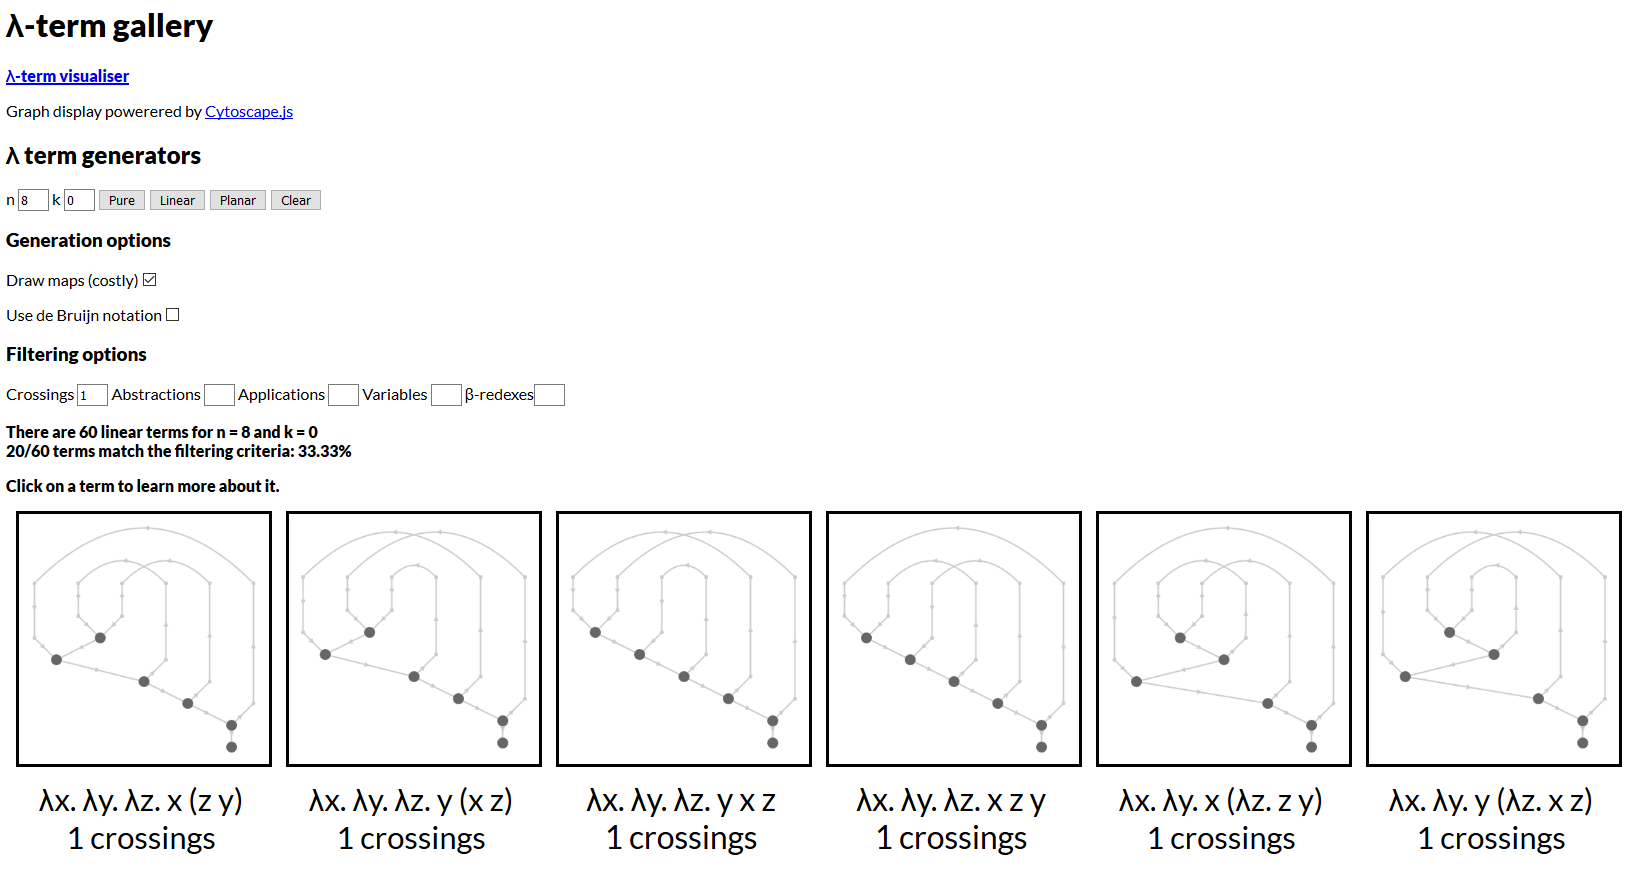
\includegraphics[scale=0.3]{gallery}
    \caption{The $\lambda$-term gallery, displaying all closed linear terms of size 5.}
    \label{fig:gallery}
\end{figure}

\subsection{Report structure}
The rest of the report is strictured as follows. Section \ref{sec:background} provides the necessary background information for the project. Section \ref{sec:features} details the features of the tools, and Section \ref{sec:implementation} details the implementation choices that went into developing them. Section \ref{sec:design} covers the design choices made during the project. Section \ref{sec:evaluation} covers the evaluation of the project, and Section \ref{sec:project-management} details how the project was managed. Appendix \ref{sec:file-structure} details the file structure of the submitted ZIP file.

\newpage

\section{Background}
\label{sec:background}

\subsection{The \texorpdfstring{$\lambda$}{lambda}-calculus}
The $\lambda$-calculus is a model of computation where programs are represented by variable abstraction and function application. It is the basis of all functional programming languages. This section will cover some concepts and terminology that will be used in the remainder of the report.

\subsubsection{Definitions}
\label{sec:defs}

The simplest terms in the $\lambda$-calculus ($\lambda$-terms) are just \textbf{variables} ($x, y, z, ...$). More complex terms can be created using the operations of \textbf{abstraction} ($\lambda x. T$) and \textbf{application} $(T_1 T_2)$. For clearer notation, applications are left-associative and abstractions extend as far to the right as possible:
%
\begin{align*}
    x \, y \, z &\equiv (x \, y) \, z \\
    \lambda x. x \, \lambda y. y &\equiv (\lambda x. x \, (\lambda y. y))
\end{align*}
%
Variables in the $\lambda$-calculus can be \textbf{bound} or \textbf{free}. A variable is bound if it is inside the scope of a corresponding $\lambda$-abstraction (it is a local variable), or free otherwise. In $\lambda x. x \, y$, the $x$ is bound but the $y$ is free. A $\lambda$-term with no free variables is called a \textbf{closed term}. Two $\lambda$-terms are said to be \textbf{$\alpha$-equivalent} if the only difference between them is the names of their bound variables -- for example, $\lambda x. x$ and $\lambda y. y$ are $\alpha$-equivalent. The process of renaming bound variables is known as \textbf{$\alpha$-conversion}:
%
$$\lambda x. T \to_\alpha \lambda y. T[x \mapsto y]$$
%
To avoid ambiguity between $\alpha$-equivalent terms, we can use \textbf{de Bruijn notation}. Rather than using explicit variable names, each variable is instead represented by how 'far away' the corresponding abstraction is. For example, $\lambda x. \lambda y. \lambda z. x \, y \, z$ can be written as $\lambda\lambda\lambda \, 2 \, 1 \, 0$. This eliminates the need for $\alpha$-conversion, and makes it much easier to implement checking for equality between $\lambda$-terms.

$\lambda$-terms contain a number of \textbf{subterms}, defined as:
%
\begin{align*}
    subterms(x) &= 1 \\
    subterms(\lambda x. T) &= 1 + subterms(T) \\
    subterms(T_1 T_2) &= 1 + subterms(T_1) \, + \, subterms(T_2)
\end{align*}

\subsubsection{\texorpdfstring{$\beta$}{Beta}-reduction}

Program execution in the $\lambda$-calculus is performed through \textbf{$\beta$-reduction} -- applying functions to their arguments. A term of the form $(\lambda x. T_1) \, T_2$ is called a \textbf{$\beta$-redex} and can be $\beta$-reduced as follows:
%
$$(\lambda x. T) \, u \to_\beta T[x \mapsto u]$$
%
Repeatedly performing $\beta$-reduction on a term until it contains no $\beta$-redexes is known as \textbf{normalisation}. A term with no $\beta$-redexes is in its \textbf{normal form}. If there are multiple $\beta$-redexes in a term, the order they are reduced in does not matter -- the same normal form will be reached. This is known as the \textbf{Church-Rosser theorem} (\cite{churchrosser}). The normal form of a $\lambda$-term is necessarily unique if it exists. However computing if normalising a pure term will terminate is undecidable \cite{church}. This is because attempts to reduce them may lead to a loop or just continuous expansion. One well-known example is the $\Omega$ term:
%
$$ \Omega = (\lambda x. x \, x)(\lambda x. x \, x) \rightarrow_\beta (x \, x)[x \mapsto (\lambda x. x \, x)] \equiv (\lambda x. x \, x)(\lambda x. x \, x) \equiv \Omega $$
%
When it is possible to get stuck in one of these normalisation loops, the order of reduction can actually matter, as shown by the example below, where reducing redex 1 leads to a new term whereas redex 2 leads to the same term:
%
$$ T = \underbrace{(\lambda x. \lambda y. x) \, a}_\text{redex 1} \, \underbrace{((\lambda x. x \, x) (\lambda x. x \, x))}_\text{redex 2} $$

$$ T \rightarrow_{\beta1} (\lambda y. a)((\lambda x. x \, x)(\lambda x. x \, x)) \rightarrow_\beta a$$
%
$$ T \rightarrow_{\beta2} (\lambda x. \lambda y. x) \, a \, ((\lambda x. x \, x)(\lambda x. x \, x)) \equiv T$$
%
The choice of which redex to reduce is related to \textbf{evaluation strategies}. Choosing the \textbf{outermost reduction} corresponds to \textbf{normal order} evaluation, in which arguments are substituted into a function before they are evaluated. Conversely, chosing the \textbf{innermost reduction} corresponds to \textbf{applicative order} evaluation, where arguments are fully evaluated before being applied to functions. Always choosing the outermost reduction is guaranteed to find the normal form if it exists. This is not the case for choosing the innermost reduction since an argument that is not used in a function could contain a normalisation loop.

The process of normalisation can be represented by \textbf{normalisation graphs}, which show the various paths between a $\lambda$-term and its normal form. An example of normalisation graphs can be seen in Figure \ref{fig:normgraphs} and \ref{fig:normgraphs2}.

\begin{figure}
    \centering
    \includegraphics{reduction}
    \caption{An example of two normalisation graphs, showing the steps of reduction taken for the terms $\lambda x. (\lambda y \, x) (\lambda z. z)$ and $\lambda x. (\lambda y. y) ((\lambda z. z) \, x)$ to reach their normal forms. Note that the diverging paths in the right example still lead to the same normal form, as stated by the Church-Rosser theorem.}
    \label{fig:normgraphs}
\end{figure}

\begin{figure}
    \centering
    \includegraphics[scale=0.4]{norm2}
    \caption{Normalisation graphs, showing the steps of reduction taken for the terms for the terms $(\lambda x. x \, x)(\lambda x. x \, x)$ and $(\lambda x. \lambda y. x) \, a \, ((\lambda x. x \, x)(\lambda x. x \, x)$, showing the normalisation loops that can occur.}
    \label{fig:normgraphs2}
\end{figure}

\subsubsection{Fragments of the \texorpdfstring{$\lambda$}{lambda}-calculus}
The \textbf{pure $\lambda$-calculus} contains all terms formed from combining variables, abstractions and applications. However we can restrict ourselves to smaller \textbf{fragments} of the $\lambda$-calculus. The \textbf{linear $\lambda$-calculus} is a subset of the pure $\lambda$-calculus containing terms in which variables are used exactly once, and the \textbf{planar $\lambda$-calculus} is a subset of the linear $\lambda$-calculus in which variables are used in the order they are abstracted in. 

Linear and planar terms have special properties relating to normalisation. Linearity and planarity are preserved by $\beta$-reduction, and all linear and planar $lambda$-terms have a computable normal form. This is because as each variable in a linear term only occurs once, terms can only get smaller with each $\beta$-reduction -- they cannot 'blow up'. Similarly, all paths to the normal form are the same length -- because all abstracted variables \textit{must} be used, there are no 'shortcuts' to the normal form by choosing a specific redex. 

It can be shown that the normal form of a linear $\lambda$-term is computable in polynomial time. To normalise a linear term, a search must be performed through the term to try and find a $\beta$-redex $(\lambda x. t)u$. Inside this $\beta$-redex, there will only need to be one substitution -- replacing the single occurrence of the abstracted variable $x$ in $t$ with the applied subterm $u$. Using the definitions of $subterms(t)$:
%
\begin{align}
    subterms((\lambda x.t)u) &= 1 + (1 + subterms(t)) + subterms(u)) \label{betabefore}\\
    subterms(t[x \mapsto u]) &= subterms(t) - 1 + subterms(u) \label{betaafter}
\end{align}
%
By subtracting \ref{betaafter} from \ref{betabefore}, we can see that the number of subterms always shrinks by three in a $\beta$-reduction. Therefore, the most reductions that a linear $\lambda$-term can have before reaching a normal form (i.e. if the term reduces to a lone variable with one subterm) is $\frac{n}{3}$. In the 'worst case' scenario, a program attempting to normalise a linear $\lambda$-term would have to normalise $n$ terms, taking $\frac{n}{3}$ operations each time. So the upper bound of complexity of normalising linear $\lambda$-terms in in $\mathcal{O}(n^2)$ -- polynomial time.

It has also been shown by \cite{mairson} that normalising linear $\lambda$-terms is PTIME-complete, by encoding boolean circuits as $\lambda$-terms. By reducing the Circuit Value Problem (known to be PTIME-complete) to normalising linear $\lambda$-terms, this proves that the latter is also PTIME-complete.

Since all planar terms are also linear terms, they share this upper bound of normalisation complexity. However, there may be a lower bound of complexity that is unknown to us. We cannot use Mairson's boolean circuits to prove this since the functions are not planar.

Linear and planar terms also have properties related to maps, which will be detailed in the next section.

\begin{table}
    \centering
    \begin{tabular}{|c|c|c|c|}
        \hline
        \textbf{Term} & \textbf{Pure} & \textbf{Linear} & \textbf{Planar} \\
        \hline
        $\lambda x. x$ & Yes & Yes & Yes \\
        \hline
        $\lambda x. (\lambda y. y) \, x$ & Yes & Yes & Yes \\
        \hline
        $\lambda x.\lambda y. x \, y$ & Yes & Yes & Yes \\
        \hline
        $\lambda x. \lambda y. y \, x$ & Yes & Yes & No \\
        \hline
        $\lambda x. x \, x$ & Yes & No & No \\
        \hline
    \end{tabular}
    \caption{Examples of terms in various fragments of the $\lambda$-calculus.}
    \label{tab:fragments}
\end{table}

\subsection{Graphs and maps}

\begin{figure}
    \centering
    \includesvg{maps}
    \caption{These two diagrams represent the same graph but two distinct maps (the ordering of edges around the point on the circle is changed). Adapted from {\cite{graphs}}}
    \label{fig:maps}
\end{figure}

In graph theory, a \textbf{graph} is a set of nodes and edges that link pairs of nodes. When these graphs are \textbf{embedded} onto a surface they are called \textbf{maps}. Unlike graphs, the order of edges around a node is important for maps, and the same graph can be represented as many different maps (an example is shown in Figure \ref{fig:maps}). A map has a \textbf{genus} which is how many 'holes' the surface it is embedded into has. \textbf{Planar maps} are maps with no crossings of edges -- they have a genus of 0. 

In this project we are particularly interested with \textbf{rooted 3-valent maps}. The \textbf{valency} of a node is how many edges connect to it - maps where all of the nodes have a valency of 3 are called \textbf{3-valent}. We can make a \textbf{rooted map} by adding a 'special' node (the \textbf{root}) that connects to the map at one point, as shown in Figure \ref{fig:trivalentrooted}.

\begin{figure}
    \centering
    \includegraphics[scale=0.3]{torus}
    \caption{An example of how a graph with crossings can be embedded onto a torus. From \shortcite{zeil4ct}.}
    \label{fig:torus}
\end{figure}

\begin{figure}
    \centering
    \includesvg[scale=0.5]{trivalentrooted}
    \caption{A 3-valent map, and the same map but rooted (root indicated by the white node)}
    \label{fig:trivalentrooted}
\end{figure}

\begin{figure}
    \centering
    \includegraphics[scale=0.6]{absapp}
    \caption{An abstraction and an application, represented as nodes of a map.}
    \label{fig:absapp}
\end{figure}

\begin{figure}
    \centering
    \includegraphics[scale=0.7]{lambdatermandgraph}
    \caption{A representation of the term $\lambda x. \lambda y. \lambda z. x \, (y \, z)$ as a rooted 3-valent map, without and with node labels. From \protect\cite{zeiljfp}.}
    \label{fig:lambdatermandgrapht}
\end{figure}

We can represent $\lambda$-terms as maps. Abstractions and applications are represented as nodes, as shown in Figure \ref{fig:absapp}. With the addition of a root to represent the start of the term, these nodes can be combined to create a rooted map, as shown in Figure \ref{fig:trivalentrooted}.

Viewing these $\lambda$-term maps can be interesting for many reasons. We can tell which terms are linear since their corresponding maps are 3-valent -- abstracted variables are only used once. Planar terms correspond to planar graphs with no crossings.

\newpage

\section{Features}
\label{sec:features}

\subsection{Drawing \texorpdfstring{$\lambda$}{lambda}-terms}
The core feature of the tools is the ability to represent any $\lambda$-term from user input as a rooted map on the screen. A context of free variables can also be specified, allowing these variables to be used in the visualised term. The user can pan and zoom around the map to inspect it more closely. Nodes can also be dragged around to new positions. The user can also choose to display the visualisation with or without labels (if just the structure is of interest). 'Full screen' mode is available so the visualised terms can fill the screen.

To make it easier to input large expressions, users can associate them with \textbf{aliases} (e.g. $id = \lambda x. x)$. A large amount can be pasted in at once with the 'bulk alias' function, which can be useful when using a large amount of predefined functions (such as Mairson's encodings of boolean circuits).

A number of properties are shown alongside the visualised term. Of most interest are the number of crossings and number of $\beta$-redexes.

\subsection{Normalisation}

The $\beta$-redexes in the term are listed next to the term when it is visualised. By hovering over them, a user can see them highlighted in the visualisation and within the term itself. Different redexes are highlighted in different colours to distinguish between them clearly. By clicking a redex, it will be performed and the visualisation updated with the newly reduced term. By continuing to click on redexes the normal form (if it exists) can be eventually reached.

Rather than clicking on the redexes, the process can be animated. There are three strategies provided: left-to-right outermost, right-to-left innermost, and random. The visualiser will highlight the redex it is about to perform, then perform it. This process repeats until the normal form is reached (or might just continue forever if there is no computable normal form).

A normalisation graph can also be generated. By default, this shows the map for each possible reduction, however this can be disabled and replaced with a blank node for large graphs since it can take a long time to render. Path lengths (shortest, longest, average etc) can also be generated.

\subsection{Generating \texorpdfstring{$\lambda$}{lambda}-term galleries}
Galleries of $\lambda$-terms with a given number of subterms and free variables can be generated. These galleries display all the maps for these terms in a grid. Captions can be shown in regular or de Bruijn notation. For larger galleries, the maps can be turned off to save time when generating them. 

By clicking on one of the 'portraits' in the gallery, the user will shown what what they would have seen had they typed that term into the visualiser.

The results can be filtered by a number of properties, such as crossings and $\beta$-redexes. The number of these terms and the proportion from the full set of terms is displayed.

\newpage

\section{Implementation}
\label{sec:implementation}

This section will cover the implementation of the tools, and issues that rose.

\subsection{Language}
To implement the tools, I decided to use \textsc{Javascript}. This was so the tools could be distributed as 'web apps' and hosted on a website rather than having to be downloaded and relying on any dependencies.

\subsection{Implementing the \texorpdfstring{$\lambda$}{lambda}-calculus in \textsc{Javascript}}
\label{sec:implementation-lambda}
The first part of developing the project was to implement the $\lambda$-calculus in \textsc{Javascript}, as a basis for the rest of the project to build on. The implementation partially based on the \textsc{ML} examples developed by \cite{pierce}. Variables are stored as de Bruijn indices -- this means that it is trivial to tell if terms are identical without having to perform $\alpha$-conversion. Abstractions and applications are constructed as combinations of subterms, making these $\lambda$-terms trees, where nodes may have zero (variable), one (abstraction) or two (application) children. Functionality was added later in the project so that terms can be associated with an \textbf{alias} to save time when writing out large expressions (for example, the alias \texttt{id} for the identity function $\lambda x. x$). An example of how terms can be represented can be seen in Figure \ref{fig:implementation}.

Since terms often contain free variables, a class to represent the context of a term was also created. This was effectively a wrapper for an array that contained the labels of terms currently in the context, with some extra methods to make manipulating it easier, such as determining a label from a given de Bruijn index. 

Printing the $\lambda$-terms proved to be more nuanced than expected. The de Bruijn representation of a term is constant and easy to print by traversing the $\lambda$-term tree recursively. However it is not very readable (especially in large terms) -- traditional labelled terms are much more intuitive. Originally variables stored a 'label' that could be printed instead of the index, but this proved to be quite buggy and often variables and their corresponding abstractions would display different labels (e.g. after $\alpha$-conversion). To fix this, labels were restricted to just abstractions, and when printing these labels would be added to a context. When the variables were to be printed, the index of the term would be looked up in the context and the appropriate label retrieved. This would ensure consistency (and subsequently correctness) throughout the term. 

When implementing the normalisation functionality, it became apparent that some sort of $\alpha$-conversion would still need to be implemented to avoid clashes of variables in the printed labels. A function was implemented to generate a 'canonical' set of labels, to ensure that each variable name was only used once in the term. For example, the term $(\lambda d. (\lambda h. h \, d) \, h) \, g$ with free variables $h$ and $g$ would be $\alpha$-converted to $\lambda x. (\lambda y. y \, x) \, a) \, b$. This would also be used when generating normalisation graphs later on -- redexes that led to $\alpha$-equivalent terms would have a consistent set of labels rather than juggling many different representations.

\begin{figure}
    \begin{minted}[frame=lines]{js}
    const y = new LambdaVariable(0);     
    const x = new LambdaVariable(1);      
    const app = new LambdaApplication(y, x);  
    const abs1 = new LambdaAbstraction(app, 'y');    
    const abs2 = new LambdaAbstraction(abs, 'x', 'swap'); 
    
    abs2.prettyPrint(); // prints \ \ 0 1
    \end{minted}
    \caption{How the function $swap = \lambda x. \lambda y. y \, x$ can be constructed in the \textsc{Javascript} implementation.}
    \label{fig:implementation}
\end{figure}

\subsection{Parsing terms from user input}
Initially the parser would iterate through the user input one character at a time, making note of 'special' characters (e.g. a backslash to represent a $\lambda$-abstraction, or an opening bracket to indicate the start of a subterm). It would then create the $\lambda$-term objects as it went from left to right. However the original parsing algorithm grew quite confusing, as it had to keep track of many different states (e.g. if an abstraction was in progress), and in practice elements could be more than one character long (such as longer variable names).

To make the process more intuitive, parsing was split into two distinct parts: an initial tokenising phase where the input would be split into the different tokens (e.g. $\lambda var. (\lambda y. y) \, var \implies$ \texttt{[\textbackslash,var,(,\textbackslash,y,),var)]}), and the parsing phase where these tokens would be formed into actual $\lambda$-terms. The benefit of tokenising first is that syntax errors (such as mismatched brackets or missing abstraction variables) are caught first, and the parser can iterate over tokens without having to worry about malformed terms. This also means that the parsing process is consistent even if variable names are longer than one character, as the labels can be stored as one token. 

This means that the 'special characters' the parser needs to check for are \texttt{(} and \texttt{)} for subterms, and \texttt{\textbackslash} for abstractions. Everything else is a variable, and adjacent tokens/subterms represent applications. To extend the parser to handle aliases, all that had to be added was to check tokens against the list of existing aliases, and use the corresponding function body if one existed.

\subsection{Drawing the terms}

To create the elements in the maps, the term is traversed recursively and new node objects are created when encountering an abstraction or application, with an edge leading to the previous parent node. When a variable is found, the appropriate edge is created between the parent node and the corresponding abstraction node. The array of map elements is then passed to the Cytoscape API (\url{http://js.cytoscape.org/}) which then generates the map.

\begin{figure}
    \centering
    \includegraphics[scale=0.17]{maps}
    \caption{How the map for the term $\lambda x. \lambda y. \lambda z. x \, (y \, z)$ evolved over time. Maps 1 and 2 are incorrect due to too many crossings, Maps 3 is correct but not aesthetically pleasing, Map 4 is the final (correct) version.}
    \label{fig:drawn_maps}
\end{figure}

\begin{figure}
    \centering
    \includegraphics[scale=0.17]{maps2}
    \caption{How the map for the term $\lambda x. \lambda y. x \, (\lambda a. \lambda b. b \, a) \, y$ evolved over time. Maps 1 is incorrect due to a lack of crossings, Map 2 is incorrect due to too many crossings, Map 3 is not only incorrect due to too many crossings but is also very hard to decipher, Map 4 is the final (correct) version.}
    \label{fig:drawn_maps2}
\end{figure}

Developing a suitable way of drawing the $\lambda$-term maps was the first major problem in the project. Drawing correct maps by hand is quite intuitive as one can place nodes and their edges 'on the fly' so that they do not cross over. However implementing an algorithm for a computer to generate these maps is significantly more difficult. Algorithms that work for some maps may not work for others, so a strategy that generates consistent maps is required. Figures \ref{fig:drawn_maps} and \ref{fig:drawn_maps2} show how the drawn map for two different terms evolved over time.

Initially maps were generated using a default layout provided by the graph drawing API (1). This placed nodes in a circle and drew the edges as the shortest path between pairs of nodes. While this representation was tidy and efficient, it did not preserve the cyclical order of edges around nodes, so the generated maps were not correct. This was due to the edges representing the use of abstracted variables 'cutting across' the map rather than exiting nodes at the right position. This caused crossings to occur for planar term maps (such as in Figure \ref{fig:drawn_maps}.1). Since edges were always straight unless there were duplicate edges between two nodes, incorrect crossings would also be generated when an edge should have curved around a node to 'dodge' an edge it but instead cut straight through it. It was clear from this method that node positions would have to be explicitly set to ensure the correctness of these maps.

In the next algorithm (2), nodes were placed progressively further up the page, with the root at the bottom. To preserve the cyclical order of edges, the scope of abstractions would always be positioned to the left of an abstraction node, and the left and right hand sides of application would be placed to the left and right respectively. To ensure that variable edges would also preserve this ordering, an extra 'support' node was added to pull a variable edge in the right direction. The edges from these support nodes and their corresponding abstraction node was changed to a bezier curve, with the intention that these edges would curve around the side of the map and only cross other variable edges when they were supposed to. Unfortunately, the edges still tended to incorrectly cross over other edges due to an insufficiently large curvature. Variables used earlier in the term would not be high up enough on the page to curve around the remainder of the term (seen in Figure \ref{fig:drawn_maps}.2) This most commonly happened with terms containing multiple larger subterms, as variables used earlier in the term would cross over edges leading to the subterms (seen in Figure \ref{fig:drawn_maps2}.2 -- the only incorrect crossing is created with the edge leading to the $\lambda a. \lambda b. b \, a$ subterm).

After looking into how the bezier curves were drawn, the algorithm was modified slightly for the next version (3). The variable support nodes were placed at the top of the page, with variables used earlier in the term having higher placed support nodes. This was so that the curves would, in theory, avoid the edges created by the rest of the term and only create correct crossings when approaching the abstraction nodes. The support nodes were also given a more subtle style so as not to be confused with the actual nodes of the map. The algorithm appeared to be successful in initial testing (in Figure \ref{fig:drawn_maps}.3), even if it produced slightly ugly maps (e.g. the 'spikes' created by the meeting of the curved edges with the straight ones). However testing with more complex terms (such as in Figure \ref{fig:drawn_maps2}.3) revealed huge flaws in the algorithm when dealing with closed subterms. The naive way that earlier variables were placed higher up the page meant that the variables used in the closed subterm were dragged downwards and caused edges to display messily and causing even more incorrect crossings. An oddity in how the curvature of variables edges were rendered can also be seen in Figure \ref{fig:drawn_maps2}.3 -- the edge representing $x$ has an unnecessarily huge curve, suggesting that the method for calculating the curvature of edges was slightly bugged too.

Since these algorithms were not having much success and the code was growing out of control, it was abandoned and started from scratch (4). Rather than diving straight into creating a new algorithm, I spent some time thinking about a strategy for drawing maps that would work for all terms. Nodes would be drawn in a similar way to before, with the scope of an abstraction heading left of an abstraction node, and the left and right hand side of an application heading out of the appropriate side. This time, however, all of the variable support nodes would be placed at the same height on the top of the page. Support nodes were also added for abstraction nodes, at the same height. This meant that any crossings would only occur at the top of the page, rather than the edges intersecting other parts of the map. The curvature radius was calculated dynamically, based on the distance between the abstraction support node and the variable support node -- the further apart they were, the greater the radius. This can be seen in Figure \ref{fig:drawn_maps}.4 -- the $x$ edge has the largest radius since it has the furthest to travel. This ensures that all three variable edges do not cross and results in a correct planar map.

Special care was also taken for positioning of subterms. All nodes inside a subterm would be shifted left or right so that they did not intersect with other parts of the map. This is shown in Figure \ref{fig:drawn_maps2}.4 -- the subterm $\lambda a. \lambda b. b \, a$ has been shifted so it is entirely right of its parent application node, and this application node has also been shifted to the right so that there is enough free space to hold the subterm.

While developing the map-generating algorithm, a recurring problem was labelling edges and nodes correctly. In the API, each element must have a unique \textit{id}, which is used when giving edges a source and target. These ids were added to a $\lambda$-context when an abstraction node was encountered so they could be looked up when variables were used later in the term. This caused problems when variable names were used multiple times in a term (such as in $\Omega = (\lambda x. x \, x)(\lambda x. x \, x)$), since uses of the second $x$ would draw edges to the first $x$. Originally, terms were $\alpha$-converted during the algorithm (e.g. $\Omega \mapsto (\lambda x. x \, x)(\lambda x'. x' \, x')$), to ensure all variable names were unique. However this meant that the labels on the generated map wouldn't match up with the term specified by the user, potentially making it confusing. Instead, a \textit{label} field was created in map elements to store the original variable name in. This meant that the \textit{id} of each element could still be unique while retaining the original label. To ensure that variable edges were drawn to the correct abstraction node, these labels were also added to the $\lambda$-context alongside the ids.

Another problem lay in how to deal with free variables. Normally when encountering a variable, it was easy to determine the appropriate abstraction node by prefixing the variable label with a $\lambda$. For free variables, this did not work at first because this abstraction node didn't exist! This meant it had to be created during the algorithm, resulting in a clumsy if statement checking for the existence of such a variable and creating a node for it if it didn't exist. This caused all sorts of bugs, such as with labelling as discussed in the previous paragraph. It turned out there was a much simpler solution to this problem -- create all the free variable nodes at the very beginning of the algorithm, so they could be treated as ordinary abstraction nodes. Initially these free variables were placed at the top of the page with the rest of the variable edges, but this caused problems when manipulating the maps later as the free and bound abstractions had different named edges. Free variables were changed to use the same basic structure as regular abstractions to ensure consistency for this reason. This provided an important lesson to ensure consistency as much as possible throughout the project so that adding new features later could be done with one block of code rather than have to adjust it for different aspects.

%% The bit above is a bit unwieldy

\subsection{Enumeration and generation functions}
The next stage of the project was to develop functions to count and generate $\lambda$-terms of various fragments of the $\lambda$-calculus. These could then be combined with the visualiser to create $\lambda$-term galleries.

The number of $\lambda$-terms with a given number of subterms $n$ and free variables $k$ can be defined as:
%
\begin{equation*}
\begin{split}
    count(n, k) = & \, count(n-1,k+1) \\
                & + \sum_{n_1 = 1}^{n - 2} count(n_1, k) \cdot count(n - 1 - n_1, k) \\
                & + [n = 1] \, k
\end{split}
\end{equation*}
%
where $[n = 1] \, k$ is equal to $k$ if $n = 1$, $0$ otherwise. 

The three terms in the sum correspond to abstractions, applications and variables respectively. The number of abstractions can be calculated by counting all terms with one less subterm (the abstraction itself counts for one subterm) and one extra free variable (the abstracted variable). The number of applications is slightly more complicated: we need to account for every possible way of splitting the subterms between the two terms $t_1$ and $t_2$. The number of variables is equal to the number of free variables, but only if the number of subterms is equal to 1 -- variables can only have one subterm, themselves!

It is quite simple to develop this equation into a program to generate $\lambda$-terms. An example in \textsc{Haskell} is shown in Figure \ref{fig:gen}. With some modifications to how we use free variables, we can also create programs to generate planar and linear terms. For planar terms, the context of free variables will be split between the LHS and the RHS of an application, so the algorithm will have to take into account the various points at which it can be split (e.g. for $\Gamma$ = \texttt{[0,1,2]}, the possibilities are \texttt{[0],[1,2]} and \texttt{[0,1],[2]}). Linear terms are slightly more complex, since the order of the context is not necessarily preserved by the two terms of an application. All the different ways the variables can be split between the LHS and RHS must be considered.

\begin{figure}
\begin{minted}[frame=lines]{haskell}
data Term = Abs Term | App Term Term | Var Int

gen :: Int -> Int -> [Term]
gen 0 _ = []
gen 1 k = [Var x | x <- [1..k]]
gen n k = [Abs t | t <- gen (n-1) (k+1)]
                ++ [App t1 t2 | 
                      n1 <- [1..n-2], t1 <- gen n1 k, 
                                        t2 <- gen (n-1-n1) k] 
\end{minted}
\caption{A program to generate pure $\lambda$-terms of a given number of subterms and free variables.}
\label{fig:gen}
\end{figure}

To test that these algorithms were in fact correct, I compared the outputs on the counting algorithms to known sequences on the \href{https://oeis.org}{Online Encycopedia of Integer Sequences (OEIS)}. For example, the sequence of numbers of closed linear $\lambda$-terms of size $n$ (generated by \texttt{[count n 0 | n <- [1..]]} forms the sequence \texttt{[0,1,0,0,5,0,0,60,0,0,1105,...]} which corresponds to sequence \href{https://oeis.org/A062980}{A062980} on the OEIS (\cite{zeiljfp}).

Translating these programs from \textsc{Haskell} to \textsc{Javascript} so they could be used by the tools was fairly simple -- pattern matching was replaced by switch statements and list comprehensions by for loops.

\subsection{The gallery}
With the term generation functions implemented in \textsc{Javascript}, the next step was to create 'galleries' to display various sets of terms in. The first thing to consider was the different parameters that could be used to filter terms to create different galleries. The original parameters $n$ and $k$ used in the generating algorithms could be used as a starting point, but there were others too such as number of crossings or number of $\beta$-redexes. There may be ways to modify the generation algorithms to only return these terms, but to start with all terms for a given $n$ and $k$ were generated, then the appropriate terms selected using a \texttt{filter(x -> ...)} call on the array. This has the downside of being quite inefficient when it comes to larger arrays of terms but meant that more time could be spent on implementing the tools rather than attempting to devise more algorithms.

Combining the visualiser with the generation algorithms was fairly easy. After receiving user input for values of $n$ and $k$, the appropriate generation algorithm (pure, linear or planar) would be run to produce an array of $\lambda$-terms. These terms could then be fed to the visualiser to produce maps of each of these terms, which would be displayed on screen using basic CSS to arrange them in a grid. Over time the way the gallery was displayed was tinkered with to ensure the best display for all displays and galleries (e.g. terms not too close together, spaced evenly etc). The ability to select filtering criteria was also added later on. One modification made to save time when generating galleries of closed terms was to infer an empty $k$ box as a 0.

A minor problem was found when passing the generated terms to the visualiser. The generated terms did not contain any labels so the visualiser treated every variable as a free variable and didn't connect the edges to the correct abstraction nodes. This was solved by giving abstracted variables unique dummy labels so the visualiser could distinguish between different abstractions.

Originally the captions for the portraits were displayed in de Bruijn notation, to represent the 'structure' of the generated terms rather than associate them with any particular labels. However, this made the captions harder to understand than regular notation. This was fixed by using the labelling function detailed in Section \ref{sec:implementation-lambda} to generate a 'canonical' labelling to display alongside the maps. An option to toggle between de Bruijn and regular notation was added, as shown in Figure \ref{fig:galleries}.

\begin{figure}
    \centering
    \includegraphics[scale=0.25]{galleries}
    \caption{The gallery showing all closed linear terms with 5 subterms, with captions in de Bruijn (top) and their regular 'canonical' (bottom) notation.}
    \label{fig:galleries}
\end{figure}

As the galleries were tested more it became apparent that for larger galleries, it simply wasn't feasible to display all the maps in a suitable time. Since the actual map-drawing process was the most computationally expensive, an option was added to turn off the map drawing and just show the captions for each term. This meant that a user would still be able to generate the terms, and inspect them in more detail by viewing their 'portrait', as discussed in the next section. 

\subsection{\texorpdfstring{$\lambda$}{Lambda}-term 'portraits'}
While the galleries were interesting alone to compare the similarities and differences between terms with the same properties, it was hard to inspect the terms in detail from the small portraits. To remedy this, functionality was added so that users could click on a portrait and be shown a larger version, similar to the first visualiser tool.

As in an actual art gallery, I thought it would be interesting to have some facts about the term displayed next to the large portrait. One of the most interesting topological properties of the maps is crossings, so an algorithm to calculate the number of crossings in a given $\lambda$-term had to be implemented. The only edges that cause crossings are those that represent the use of abstracted variables. For a map to have no crossings, its variables must be used in the order they are abstracted, i.e. their de Bruijn indices read from left to right must be in descending order. So to find the crossings created by a particular variable, we can calculate $crossings(x) = |x - (n - 1 - i)|$, where $x$ is the de Bruijn index of the variable, $n$ is the length of the context, and $i$ is the position of the variable in the context. For example, in a list of free variables \texttt{[0,1,2]}, the \texttt{0} creates two crossings as it must pass through the edges for variables \texttt{1} and \texttt{2}. Unfortunately, we cannot just perform this calculation for each variable and add them together to find the total number of crossings since this would contain duplicate crossings. 

To solve this problem, a slightly different approach was used. This approach was based on the idea that a crossing is created when a free variable on the LHS of an application has a lower de Bruijn index than a variable on the RHS. For example, $0 \, (1 \, 2)$ has two crossings because $0$ is less than both variables in the RHS, whereas $2 \, (1 \, 0)$ has no crossings since $2$ is greater than both variables in the RHS. These crossings could then be added to the crossings in the LHS and RHS by recursively applying the algorithm. A pseudocode implementation of the calculation of crossings in an application can be seen in Figure \ref{fig:crossings}. It is trivial to consider the other two cases: variables have no crossings and abstractions have the same number of crossings as their scope.

There was initially some trouble translating this into \textsc{Javascript} as I made a severe lapse of judgement and tried to incorporate calculating the free variables into the crossings function. Since \textsc{Javascript} does not contain tuples, this meant performing various array manipulation options to keep track of the current number of calculated crossings and free variables in the same array -- this made the function very hard to understand! I realised that to keep the code cleaner it would be better to first implement a separate function to return an array of free variables in a $\lambda$-term. This made the crossings function much tidier and the implementation become very close to the algorithm in Figure \ref{fig:crossings}.

\begin{figure}
\begin{algorithm}[H]
    \SetKwArray{LHS}{freeLHS}
    \SetKwArray{RHS}{freeRHS}
    \SetKwData{TotalCrossings}{totalCrossings}
    \SetKwFunction{freeVariables}{freeVariables}
    \SetKwFunction{Crossings}{crossings}
    \SetKwFunction{length}{length}
\LHS $\leftarrow$ \freeVariables{LHS} \;
\RHS $\leftarrow$ \freeVariables{RHS} \;
\TotalCrossings $\leftarrow$ \Crossings{LHS} $+$ \Crossings{RHS} \;
\For{$i \leftarrow 0$ \KwTo \length{\LHS}}{
    \For{$j \leftarrow 0$ \KwTo \length{\RHS}}{
        \If{\LHS{i} $<$ \RHS{j}}{
            \TotalCrossings $\leftarrow$ \TotalCrossings + 1 \;
        }
    }
}
\Return \TotalCrossings \;
\end{algorithm}
\caption{Algorithm to calculate crossings in an application.}
\label{fig:crossings}
\end{figure}

Other facts about the visualised term were much simpler to implement: calculating the number of applications, abstractions and variables involved traversing the term and incrementing a counter whenever a particular element appeared.

With the $\lambda$-term portraits in good condition, I decided to add them to the visualiser as well, to create more consistency between the two tools. This also enabled code to be shared between the tools and the overall size of the codebase to decrease, making it easier to maintain.

\subsection{Interacting with \texorpdfstring{$\beta$}{beta}-redexes}
With the core functionality of the visualiser and the gallery complete, it was time to turn to more specific features. Since one of the main motivations of the project had been to investigate normalisation, $\beta$-redexes were a good area to head into next.

I again turned to the \textsc{ML} functions developed by \cite{pierce}. Firstly, a function to 'shift' all de Bruijn indices greater than a given number by a certain number of places had to be implemented, followed by a function to substitute a variable for a different term. These could then be combined to create a $\beta$-reduction function. At this point, I also made a basic normalisation function that continuously performed an outermost reduction until reaching a normal form or performing a certain number reduction steps. Combining this with the visualiser was again simple: the map drawing function could be called after reducing or normalising the original term to draw the new term.

The next feature to implement was to list the $\beta$-redexes alongside the portraits. This was just a case of traversing the term tree and adding each $\beta$-redex to an array when finding one, meaning that the leftmost outermost redex would be in position \texttt{0} and the rightmost innermost redex would be in position \texttt{n}, as shown below:
%
$$ \overbrace{(\lambda x. \underbrace{(\lambda y. y) \, x}_\text{redex 1}) \, (\lambda x. \underbrace{(\lambda y. y) \, x}_\text{redex 2})}^\text{redex 0} $$
%
These redexes could then be printed next to the portraits. To implement clicking on the redexes to reduce it, a function to perform a specific reduction in a term had to be implemented. This was again a case of traversing the term in the same way with a counter that ticked down until the appropriate redex was encountered.

To allow highlighting of redexes in the original term, a method to print terms with HTML tags had to be implemented. This would print the term with \texttt{<span>} tags surrounding each beta redex, so each redex was associated with a class. For example, the term $(\lambda x. x) \, a$ would be enclosed with \texttt{<span class="app-0 beta-0">...</span>}. The style for this class could then be changed when highlighting its corresponding redex in the list. 

This became slightly more complicated when dealing with redexes within other redexes -- the function to change the style of a class had change the style of all classes within the \texttt{<span>} tags since the inner classes overwrote the outer ones. This is shown in Figure \ref{fig:highlight}.

\begin{figure}
    \centering
    \includegraphics[scale=0.5]{highlight}
    \caption{An example showing how the redex highlighting originally had trouble when dealing with redexes inside redexes, and how it now correctly displays.}
    \label{fig:highlight}
\end{figure}

A similar approach was used when making the redex highlight on the map. The API used allows elements to have classes, so whenever a redex was encountered a corresponding class would be added to an array, and added to all elements within the redex. Whenever a redex was highlighted, the style function from the API could be called and update all the elements with the appropriate class with the colour.

\subsection{Normalisation graphs}
One main idea from the project proposal was the use of the visualised maps in normalisation graphs. The first step in this was to implement these normalisation graphs as a data structure in \textsc{Javascript}, and then using these structures alongside the graph drawing API to generate the graphs.

Originally normalisation graphs were created as a naive tree structure. The root node contained the original term, with children representing all possible reductions of that term (each edge representing an individual redex). While this seemed like a suitable idea in theory, it was flawed in that not all redexes lead to unique reductions (the two redexes in $(\lambda x. (\lambda y. (\lambda z. z) \, y) \, x)$ lead to $\alpha$-equivalent terms, but the tree structure could not represent two edges leading to the same node. This also meant that the normalisation graph would not converge to the normal form at the bottom, but would diverge to many nodes containing the same normal form. This implementation would also fail to detect normalisation loops and would continue to descend the tree infinitely. However it had the benefit of being simple to implement and understand.

Regardless of its problems, this implementation was used for the first iteration of generating normalisation graphs. Since the graph API had the ability to create 'compound nodes' (nodes with other graph elements inside them), the first strategy was to traverse the normalisation tree, generating maps of the terms at each node and placing them inside the larger node of the normalisation graph. The ids of elements would have to be renamed so that maps from different nodes didn't link up by mistake, but this was just a case of suffixing a unique id after each map's elements. These normalisation graph nodes would then be connected by the edges representing redexes. To place the nodes, each reduction was given a 'level' value which specified how many steps had been taken to reach it from the original term. Nodes with the same level were spread out evenly in a row, with rows starting from the top of the page and moving down. This works fine for linear terms, since steps always take you further down the normalisation graph due to all paths being the same length (it is impossible to get to another reduction on the same level). However for pure terms this can cause some irregularities since consecutive reductions can occupy the same level. Since edges are drawn in straight lines, this means they can cut across other nodes in the graph, as shown in Figure \ref{fig:purenorm}. Fortunately this doesn't happen too frequently, and the nodes can be moved out of the way of the edge if desired.

\begin{figure}
    \centering
    \includegraphics[scale=0.5]{purenorm}
    \caption{An example of when the generated normalisation graph can feature edges than cross behind other nodes for pure terms (the edge from the right node to the left node crosses behind the centre node). However it is a lot harder than expected to find examples like this.}
    \label{fig:purenorm}
\end{figure}

The first attempt at drawing normalisation graphs had numerous problems. While the API didn't redraw nodes with duplicate ids (which I thought might remove the problem of the duplicate reductions in the normalisation tree), there was a problem with edges, since each node of the tree would attempt to draw its own set of edges from the node and causing many duplicates. This was fixed by checking for unique reductions in the graph drawing algorithm, but this was unwieldy and made the algorithm quite hard to understand. Compound nodes also caused the performance of the map to drop drastically, especially when moving around nodes, which cause a lot of lag. This was not helped by each duplicate node drawing its own map, which I took a while to realise since the maps were drawn on top of each other. Finally there were no options to give a margin around the maps in the normalisation graph nodes, so some of the edges would intersect with the edge of their parent node, as shown in the left of Figure \ref{fig:normnodes}.

\begin{figure}
    \centering
    \includegraphics[scale=0.35]{nodenorm}
    \caption{A comparison between the compound node (left) and background image (right) versions of normalisation graph nodes.}
    \label{fig:normnodes}
\end{figure}

In an attempt to reduce the lag created by the drawn graph, I switched to using images for the normalisation graph nodes. The map of the reduction would be generated first, then converted to an image using the API functions. This image could then be used as the background of the normalisation graph node, as shown in the right of Figure \ref{fig:normnodes}. This made creating tidier nodes much easier as a margin could be specified around the image so everything fit inside. Options were also added to disable map generation for large terms (like with the gallery) to reduce the generation time of the graph. It also turned out that drawing arrows on the edges was a large cause of lag, so an option to not draw these was also added. 

While the tree implementation of normalisation graphs had just about been holding up through all of this tweaking, it started to show severe weaknesses when attempting to implement functions to calculate path length. Because of the numerous duplicate nodes, complex method needed to be implemented to ensure that only unique paths were being calculated. This was quite complicated and bloated the functions significantly. I decided that it was time to migrate to a more sophisticated implementation.

Rather than a tree, the new implementation uses an adjacency matrix that keeps track of which nodes connect to each other, and by which redex. The original term is fed to the initialisation algorithm, which then performs all the redexes in the term and adds the resulting reductions to a frontier. The current node is added to the adjacency matrix, with references to the nodes it connects to. This process is continued, with any previously seen reductions not being re-added to the frontier, until the frontier is empty and the graph is complete. This has several benefits over the tree implementation. Most notably, every node is unique, which also means that there are no duplicate edges that need to be removed when creating the map. Additionally, because redexes are implemented as references to already existing objects rather than new child objects, infinitely reducing terms with finite normalisation graphs (such as $(\lambda x. x \, x)(\lambda x. x \, x)$) can have these graphs displayed. The only time the algorithm could carry on infinitely would be if the term reduces infinitely with an infinite normalisation graph, such as for $(\lambda x. x \, x \, x)(\lambda x. x \, x \, x)$. For these terms, a cutoff point was added to halt the algorithm at a suitable number of reductions. In the code, the algorithm becomes much more elegant (both while generating the graph and drawing it), since recursion into the tree is replaced with a loop across the adjacency matrix. The value for 'level' was calculated in a similar way to before, with all reductions from the original term assigned level 1, and each subsequent redex increasing this value by 1.

Path functions were now easier to implement. The total number of paths and list of different path lengths could be calculated by starting at the original term and following the references in the adjacency matrix until the normal form was reached. Properties such as shortest or longest path could then be computed by performing operations on the list of path lengths, such as \texttt{min()} or \texttt{max()}.

A feature added slightly later on was the ability to hover over edges and see the redex that that it represented. The API provided functions for performing actions on mouse events, so this was easy to implement. The only minor problem was that redexes could free variables that were bound in the original term, so when it came to printing them there was no way of knowing which variable they referred to. For example, $\lambda \, (\lambda \, 0) \, 0$ prints as $\lambda x. (\lambda y. y) \, x$ but the redex $(\lambda \, 0) \, 0$ on its own prints as $(\lambda y. y) \, ?$, since the $x$ is never bound. This was solved by storing the correctly printed version of the redex at graph initialisation (by considering the original term) rather than trying to generate the label at run-time.

\subsection{Animating normalisation}
The last major feature implemented was animating the normalisation of terms. In theory, this was simple: highlight the appropriate redex, then perform it and redraw the new term, then keep going until the normal form was reached. Unfortunately, chaining these operations was slightly harder than anticipated since \textsc{Javascript} is single-threaded and as such doesn't have a conventional \texttt{sleep()} function like in multi-threaded languages. Instead it has a \texttt{setTimeout()} function that is passed a function and executes it after a given time. This meant that what was originally a simple while loop had to become a recursive function with several nested \texttt{setTimeout()} functions for the process of highlighting and performing each redex, then calling the animation function on the new term.

Three strategies were implemented: leftmost outermost, which chooses performs the first redex in the redex list, rightmost innermost, which performs the last redex in the redex list, and random.

\subsection{Finishing touches}
With all main functionality completed, all that was left to do was to polish up the interface. To make use of the tool easier, the page would automatically scroll down to the appropriate section of the page once buttons were clicked, rather than making users scroll down themselves. 

One thing I noticed was how large maps and graphs were quite hard to view, so I implemented a fullscreen mode to redraw them to fill the screen.

\newpage

\section{Design choices}
\label{sec:design}
A little bit about the design choices made for the tool?

\subsection{\texorpdfstring{$\lambda$}{Lambda}-term visualiser}


\subsection{\texorpdfstring{$\lambda$}{Lambda}-term gallery}


\newpage
\section{Evaluation}
\label{sec:evaluation}
How well does it work?

\newpage
\section{Examples}
What could it be used for?

\subsection{Visualising terms}
The main 

\subsection{Terms with infinite reductions but finite graphs}
Some terms, such as $\Omega$, have no computable normal form, but do have finite normalisation graphs. These can be generated by the visualiser. An example that combines $\Omega$ with a path that does reach a normal form is shown in Figure \ref{fig:omega}.

\subsection{Boolean circuits}
To prove that normalisation of linear $\lambda$-terms is PTIME-complete, \cite{mairson} encoded boolean circuits as functions in \textsc{ML}. By normalising these functions, the output of the boolean circuit can be produced. Since the Circuit Value Problem is known to be PTIME-complete, reducing it to the normalisation of linear $\lambda$-terms shows that the latter is also PTIME-complete.

\begin{figure}
    \centering
    \includegraphics[scale=0.4]{normgraph}
    \caption{An example of a normalisation graph with loops for the term $\lambda x. (\lambda y. \lambda z. y) \, x \, ((\lambda w. w \, w)(\lambda u. u \, u))$.}
    \label{fig:omega}
\end{figure}

It can be interesting to use the visualiser to view the structure of the maps associated with these. One example is the circuit shown in Figure \ref{fig:circuit}, which is encoded as $\lambda x.$ \texttt{Copy} $x \, (\lambda x_1. \lambda x_2.$ \texttt{Notgate} $x_1 \, (\lambda x_3.$ \texttt{Orgate} $x_3 \, x_2 \, (\lambda x_4. x_4))$. The \texttt{Copy} function represents a fanout gate, copying one input $x$ to two outputs, $x_1$ and $x_2$. The \texttt{Notgate} function takes the input $x_1$ and negates it to to the output $x_3$. The \texttt{Orgate} function takes in two inputs $x_2$ and $x_3$ and returns the \texttt{Or} of these as $x_4$.

The corresponding map is shown in Figure \ref{fig:circuitmap}, demonstrating how very simple circuits can create quite large maps! If we give the circuit an input, we use the visualiser to step through the redexes and arrive at the normal form, which will be the output of the circuit. The circuit in Figure \ref{fig:circuit} applied to \texttt{True} normalises to the pair representing \texttt{True}, as expected.

In theory, the normalisation graphs for these circuits could also be generated to view all the different paths normalisation could take. Unfortunately, this appears to be infeasible on desktop machines due to the huge number of nodes in the graph. However, the normalisation graphs for smaller terms \textit{can} be generated in a suitable time, such as the one representing \texttt{And True False} in Figure \ref{fig:andnorm}.


\begin{figure}
    \centering
    \includesvg[scale=0.75]{circuit}
    \caption{A simple boolean circuit, representing \texttt{x -> Or (Not x) x}.}
    \label{fig:circuit}
\end{figure}

\begin{sidewaysfigure}
    \centering
    \includegraphics[scale=0.4]{circuitmap}
    \caption{The corresponding map for the circuit in Figure \ref{fig:circuit}}
    \label{fig:circuitmap}
\end{sidewaysfigure}

\begin{figure}
    \centering
    \includegraphics[scale=0.25]{andgate}
    \caption{The structure of the normalisation graph for \texttt{And True False}.}
    \label{fig:andnorm}
\end{figure}

\subsection{Testing conjectures}
When tes

One very simple example of a conjecture could be \textit{All closed linear terms of size 11 with 3 $\beta$-redexes are planar}. There are 1105 linear terms of size 11, of which 14 contain three $\beta$-redexes, so even working out which terms fit the criteria would take a long time by hand, and drawing them even longer. By using the gallery, it is very simple to generate the 14 terms and verify that, indeed, they are all planar. One thing I noticed while testing the gallery is that closed linear terms of size 8 with two $\beta$-redexes and size 5 with one $\beta$-redex are also all planar, as shown in Figure \ref{fig:testingconjecture}. This could lead to the conjecture \textit{All closed linear terms of size $n$ with $\frac{n-2}{3}$ $\beta$-redexes are planar}. This also holds for size 14 with 4 $\beta$-redexes, but cannot be tested much further since my computer cannot generate larger terms in a suitable time. Nevertheless, it is a good starting point

\begin{figure}
    \centering
    \includegraphics[scale=0.23]{testingconjecture}
    \caption{Testing the conjecture \textit{All closed linear terms of size $n$ with $\frac{n-2}{3}$ $\beta$-redexes are planar}.}
    \label{fig:testingconjecture}
\end{figure}


\newpage

\section{Project management}
\label{sec:project-management}
How everything got done

\newpage
\section{Conclusion}
\label{sec:conclusion}
Conclude

\newpage

\bibliography{refs}

\newpage
\appendix

\section{File structure}
\label{sec:file-structure}
This appendix details the file structure of the submitted ZIP directory. To run either of the tools, simply load up one of the \texttt{.html} files in the root of the directory in your preferred browser.

\subsection{\texttt{root} -- Main files}
\begin{itemize}
    \item \texttt{gallery.html}: The $\lambda$-term gallery.
    \item \texttt{visualiser.html}: The $\lambda$-term visualiser.
    \item \texttt{aliases.txt}: Some sample aliases for use in the visualiser, including Mairson's boolean circuit functions, adapted from \cite{mairson}.
    \item \texttt{README.md}: A readme file.
\end{itemize}

\subsection{\texttt{docs} directory -- Documentation}
\begin{itemize}
    \item \texttt{2018-10-26-project-proposal.pdf}: The original project proposal.
    \item \texttt{2018-11-23-scientific-paper.pdf}: The scientific paper, detailing some project background and the state of the project towards the end of November 2018.
    \item \texttt{2019-04-08-final-report.pdf}: The final report (this document).
\end{itemize}

\subsection{\texttt{src} directory -- Source code}
\begin{itemize}
    \item \texttt{cytoscape.min.js}: The source code for the graph drawing API used.
    \item \texttt{definition.js}: The implementation of the $\lambda$-calculus and associated data structures.
    \item \texttt{evaluator.js}: Functions to evaluate and normalising $\lambda$-terms.
    \item \texttt{galleryFunctions.js}: Functions used in the gallery.
    \item \texttt{Generator.hs}: The original Haskell versions of the $\lambda$-term counting and generating functions.
    \item \texttt{generator.js}: Functions to count and generate $\lambda$-terms.
    \item \texttt{graph.js}: Functions to generate the $\lambda$-term maps and normalisation graphs
    \item \texttt{parser.js}: Functions to parse and tokenise user input into $\lambda$-terms.
    \item \texttt{sharedFunctions.js}: Functions shared between the gallery and visualiser.
    \item \texttt{style.css}: The style document for the two HTML pages.
    \item \texttt{visualiserFunctions.js}: Functions used in the visualiser.
\end{itemize}

\subsection{\texttt{pics} directory -- Images}
Some images of the tools in action.

\end{document}
